\section{Les particules du modèle standard}

\begin{figure}[h]
\ifdefined\homedir \else \def\homedir{/home/torterotot}\fi
\IfFileExists{\homedir/Dropbox/Enseignement/TikZ_files/modele_standard_EN/init.tex}{
\includegraphics[width=\textwidth]{\PhDthesisdir/contents/chapter-MS-MSSM/SM_ptcs/_SM2018.tex}
}{
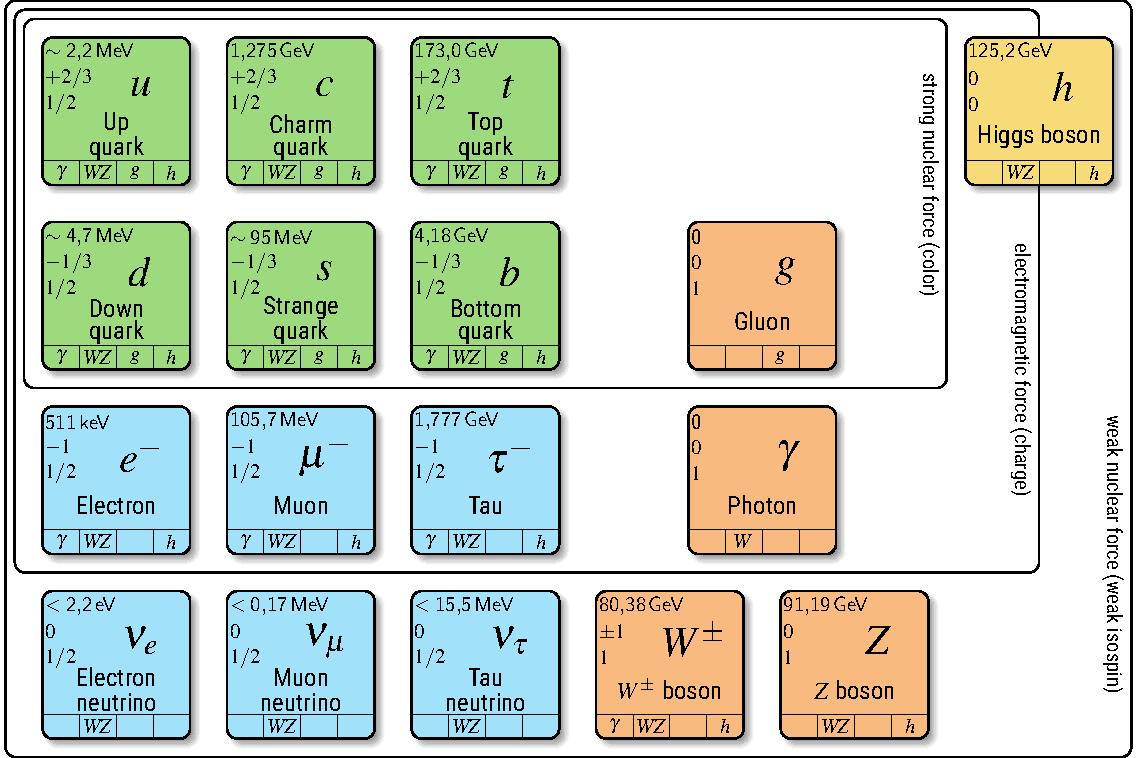
\includegraphics[width=\textwidth]{\PhDthesisdir/tex/slides/SM_MSSM_HTT_pheno/SM_and_its_limits/SM_2018-bak.pdf}
}
\caption{Les particules du modèle standard.}
\end{figure}

ptc fondamentale = ? 10e-18 m

\subsection{Les fermions}
spin demi entier (stat Fermi-Dirac). Constituants de la matière, il y en a 12.

\paragraph{Quarks} fermions avec couleur

\paragraph{Leptons}


\subsection{Les bosons}
spin entier, 1 (bosons de jauge, bosons vecteurs, vecteurs de force) ou 0 (Higgs)

\Wboson\ et chiralité?

